\normaltrue \difficilefalse \tdifficilefalse
\correctionfalse
%\UPSTIidClasse{11} % 11 sup, 12 spé
%\newcommand{\UPSTIidClasse}{11}

\exer{Hublex $\star$ \label{C2:04:68}}
%% CCINP MP 2020
\setcounter{numques}{0}
\UPSTIcompetence[2]{C2-04}
\index{Compétence C2-04}
\index{Correcteur}
\index{Correcteur proportionnel intégral}
\index{Hublex}


\ifcorrection
\else
\textbf{Pas de corrigé pour cet exercice.}
\fi


L’architecture retenue pour contrôler le couple moteur est un asservissement en intensité, image du
couple moteur (voir équation précédente). Le schéma-blocs est représenté \autoref{fig_13}. Un convertisseur IU
fournit au calculateur une tension $\indice{u}{ic}(t)$ image de l’intensité de consigne $i_c(t)$, proportionnelle à cette
dernière de coefficient $\indice{K}{iu}$. De même, l’intensité réelle $i(t)$, mesurée par un capteur d’intensité de
coefficient $\indice{K}{capt}$, a pour image $\indice{u}{im}(t)$. L’écart, noté $\varepsilon(t) = \indice{u}{ic}(t) - \indice{u}{im}(t)$, est traité par le correcteur de fonction de transfert $C(p)$, qui impose la tension $u(t)$ aux bornes du moteur.
%On note $I_c(p)$, $\indice{U}{ic}(p)$, $\indice{U}{im}(p)$, $\varepsilon(p)$ les transformées de Laplace respectives de $i_c(t)$, $\indice{u}{ic}(t)$, $\indice{u}{im}(t)$ et $\varepsilon(t)$.

On donne la fonction de transfert du moteur : $H_m(p)=K_m\dfrac{1+\tau_m p}{1+\dfrac{2z_m}{\omega_{0m}}p+\dfrac{1}{\omega_{0m}^2}p^2}$.


\begin{figure}[H]
\centering
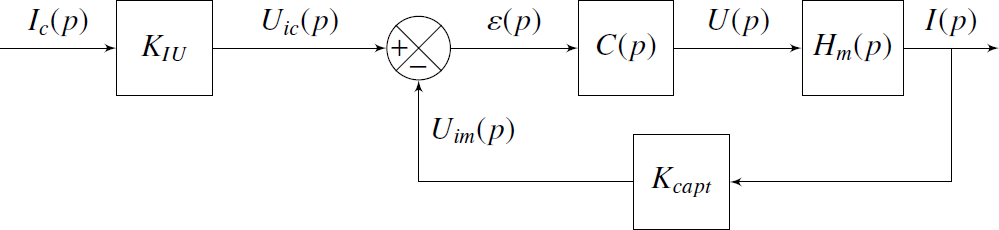
\includegraphics[width=\linewidth]{fig_13}
\caption{Schéma-blocs \label{fig_13}}
\end{figure}

\question{Préciser, en justifiant, quelle valeur donner à $\indice{K}{iu}$, caractéristique du convertisseur IU.}

On prend, dans un premier temps, un correcteur purement proportionnel: $C(p)=K_p$.

On en déduit la fonction de transfert $H_I(p)=\dfrac{I(p)}{I_c(p)}$ :

$H_I(p)=\dfrac{K'}{1+K'}\dfrac{1+\tau_m p}{1+  
\dfrac{\dfrac{2z_m}{\omega_{0m}}+ K'\tau_m}{1+K'}p 
+ \dfrac{1}{\omega_{0m}^2(1+K')} p^2}$, avec $K'=\indice{K}{iu}K_pK_m$.


\question{Calculer l’expression littérale de l’erreur en régime permanent notée $\mu_s$, pour une entrée indicielle (i.e. $I_c(p)$ est un échelon unitaire), en fonction de $\indice{K}{iu}$, $\indice{K}{p}$ et $K_m$.}

La \autoref{fig_14} présente les diagrammes de Bode en boucle ouverte de l’asservissement étudié, en prenant $K_p=10$.


%Q30.
\question{Conclure, lorsque cela est possible, quant au respect des sousexigences de l’exigence «~1.7.1.1~» avec ce type de correcteur.}

Dans un deuxième temps, il est décidé d’utiliser un correcteur de type proportionnel intégral. Sa fonction de transfert est notée : $C(p)=K_p+\dfrac{K_i}{p}$.

%Q31.
\question{Préciser l’influence de cecorrecteur sur les performances du système. Justifier le choix de ce type de correcteur dans le cas étudié.}

On souhaite régler le correcteur afin de respecter les performances de précision et de stabilité.

%Q32.
\question{Tracer sur le DR4, les diagrammes de Bode asymptotique du correcteur, ainsi que l’allure des courbes réelles pour $K_p=10$ et $K_i=1000$. On précisera les valeurs numériques associées aux valeurs caractéristiques. On se propose de régler le correcteur grâce à la méthode suivante, en deux étapes :}
\textit{\begin{enumerate}
\item réglage de $K_p$ seul (c’est-à-dire en considérant $K_i=0$ tout d’abord), de façon à respecter les exigences de stabilité et de bande passante;
\item  réglage de $K_i$ de façon à éloigner la pulsation de cassure du correcteur à une décade vers la gauche de la pulsation de coupure à \SI{0}{dB}, de manière à ce que $\SI{0}{dB}$ ne soit quasiment pas modifiée.
\end{enumerate}}

%Q33.
\question{En suivant cette méthode, déterminer en justifiant la valeur numérique de $K_p$.}

%Q34.
\question{Déterminer alors la valeur numérique de $K_i$.}

 Une fois le correcteur réglé, on obtient les diagrammes de Bode en boucle ouverte (\autoref{fig_15}) et les réponses temporelles (\autoref{fig_16}), pour un échelon d’intensité $i_c(t)$ de \SI{2}{A}.

% Q35.
\question{Commenter le résultat obtenu vis-à-vis de l’exigence «~1.7.1.1.4~». Expliquer pourquoi, à partir des exigences du D6, cet asservissement n’est pas directement implanté en l’état dans le système.}

Le correcteur reste inchangé. Afin de palier au problème identifié précédemment, on apporte une dernière évolution au sein du calculateur. Cela permet de respecter les exigences de l’asservissement. \autoref{fig_17} présente les réponses temporelles du système pour un échelon d’intensité $i_c(t)$ de \SI{2}{A}.

%Q36.
\question{Préciser quelle ultime modification a apporté le constructeur afin de respecter les exigences de l’asservissement.}


\begin{figure}[H]
\centering
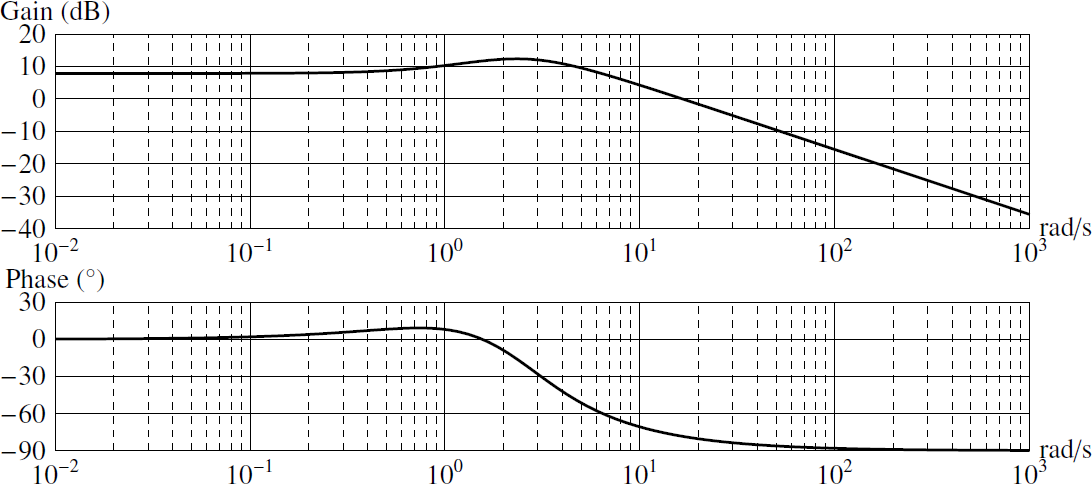
\includegraphics[width=\linewidth]{fig_14}
\caption{Diagrammes de Bode en boucle ouverte pour $K_p = 10$\label{fig_14}}
\end{figure}


\begin{figure}[H]
\centering
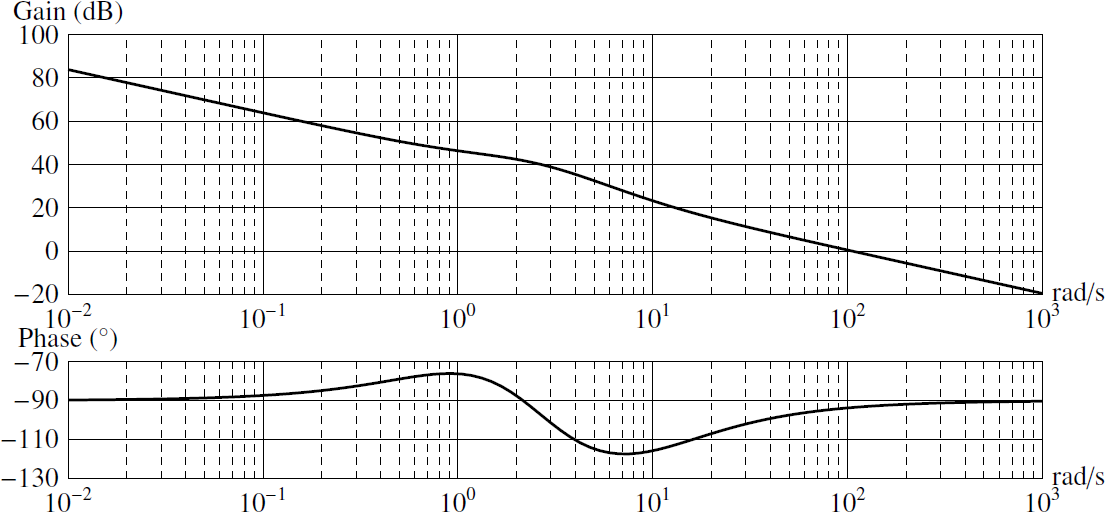
\includegraphics[width=\linewidth]{fig_15}
\caption{Diagrammes de Bode en boucle ouverte avec réglage du correcteur PI effectué \label{fig_15}}
\end{figure}

\begin{figure}[H]
\centering
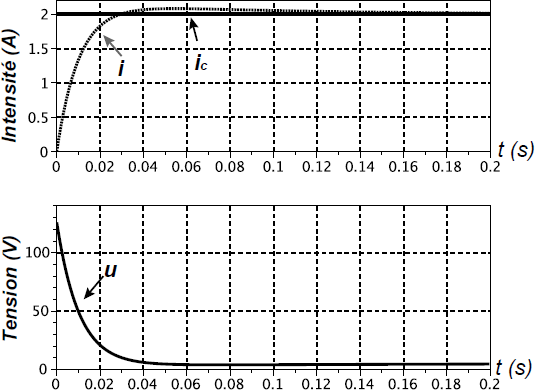
\includegraphics[width=.95\linewidth]{fig_16}
\caption{Réponses temporelles avec réglage du correcteur PI effectué \label{fig_16}}
\end{figure}


\begin{figure}[H]
\centering
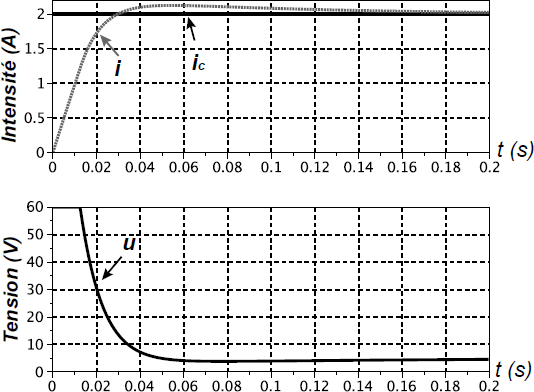
\includegraphics[width=.95\linewidth]{fig_17}
\caption{Réponses temporelles du système finalement implanté\label{fig_17}}
\end{figure}

\noindent\footnotesize
 \fbox{\parbox{.9\linewidth}{
Éléments de corrigé : 
\begin{enumerate}
\item .
\end{enumerate}}}
\normalsize

\begin{flushright}
\footnotesize{Corrigé  voir \ref{C2:04:70}.}
\end{flushright}%
\fi